%%%%%%%%%%%%%%%%%%%%%%%%%%%%%%%%%%%%%%%%%%%%%%%%%%%%
\documentclass[12pt]{article}
\usepackage{sbc-template}
\usepackage{tikz}
\usepackage{listings}
\usepackage{color}
\newcommand{\mohammad}[1]{\textcolor{red}{Mohammad: #1}}

\definecolor{dkgreen}{rgb}{0,0.6,0}
\definecolor{gray}{rgb}{0.5,0.5,0.5}
\definecolor{mauve}{rgb}{0.58,0,0.82}

\lstset{frame=tb,
	language=Python,
	aboveskip=3mm,
	belowskip=3mm,
	showstringspaces=false,
	columns=flexible,
	basicstyle={\small\ttfamily},
	numbers=none,
	numberstyle=\tiny\color{gray},
	keywordstyle=\color{blue},
	commentstyle=\color{dkgreen},
	stringstyle=\color{mauve},
	breaklines=true,
	breakatwhitespace=true,
	tabsize=3
}
%%%%%%%%%%%%%%%%%%%%%%%%%%%%%%%%%%%%%%%%%%%%%%%%%%%%


%%%%%%%%%%%%%%%%%%%%%%%%%%%%%%%%%%%%%%%%%%%%%%%%%%%%
\title{Abstraction Layer for Data Cleaning Tools}
\author{Milad Abbaszadeh Jahromi\inst{1}}
\address{Technische Universit\"{a}t Berlin \email{Milad.abbaszadehjahromi@tu-berlin.de}}
\begin{document} 
\maketitle
%%%%%%%%%%%%%%%%%%%%%%%%%%%%%%%%%%%%%%%%%%%%%%%%%%%%


%%%%%%%%%%%%%%%%%%%%%%%%%%%%%%%%%%%%%%%%%%%%%%%%%%%%
\begin{abstract} 
	This is the abstract...
	\mohammad{leave abstract. i will write it.}
		
	% \textbf{Keywords}: Keyword 1, Keyword 2, Keyword 3.
\end{abstract}
%%%%%%%%%%%%%%%%%%%%%%%%%%%%%%%%%%%%%%%%%%%%%%%%%%%%


%%%%%%%%%%%%%%%%%%%%%%%%%%%%%%%%%%%%%%%%%%%%%%%%%%%%
\section{Introduction}
\label{section:introduction}

\subsection{Motivation}
Despite the increase amount of data which is generating every  single second[1] and the value has made out of that, the data quality is even more important in compare to several decade ago. One of the ways that helps this approach is data cleaning.Although there aren't many tools that works in this area,heterogeneity and Dispersion of each tool make the process harder.Furthermore,each tool has different installation,input and output structure that can be time consuming and be catastrophic for users and forced them to stick to each tool structure that isn't desirable for most of the experts. 
This report represents the abstract layer which can help users to avoid from conflicting with the tools for cleaning purpose and help them for unique and constant input and output which can be really remarkable to save time for experts and let them to work with single and common input and output for all tools that covered by abstract layer.

\mohammad{the motivation can be so much better and stronger. talk about different tools that have heterogeneity in terms of language, installation, input/output system and so on and the user difficulties.}

\subsection{Contributions}
experts of cleaning, most of the time use cleaning tools and they don't like to get involved in installation and command usage which is required for running, you can simply use our abstract layer.
In other words because of the following reasons experts should use this abstract layer:
\begin{itemize}
	\item Simple install
	\item Easy to use
	\item Hide installation of each tool
	\item constant Input
	\item constant output 
	\item constant instructed command 
	
\end{itemize}
With this layer data has been sent as result, the Suspicious elements come up with  constant type and format which is generated as a output for each tool.

\mohammad{talk about how this module can address the so-called heterogeneities for the user's application. use bullet list just like the other papers' contributions. talk about user instead of "you".}

\subsection{Architecture}
The abstract layer located as part of user code in real world like common dictionary and it has utilized as Connector between the user's application and each tool which is consumed for cleaning purpose[figure 1] and try to hide the levels of communicating with tools.

\mohammad{in this subsection talk about the big picture of the architecture and the position of the abstraction layer in the user system. I have added a proper figure. you write the texts.}
\begin{figure}[!htb]
	\centering
	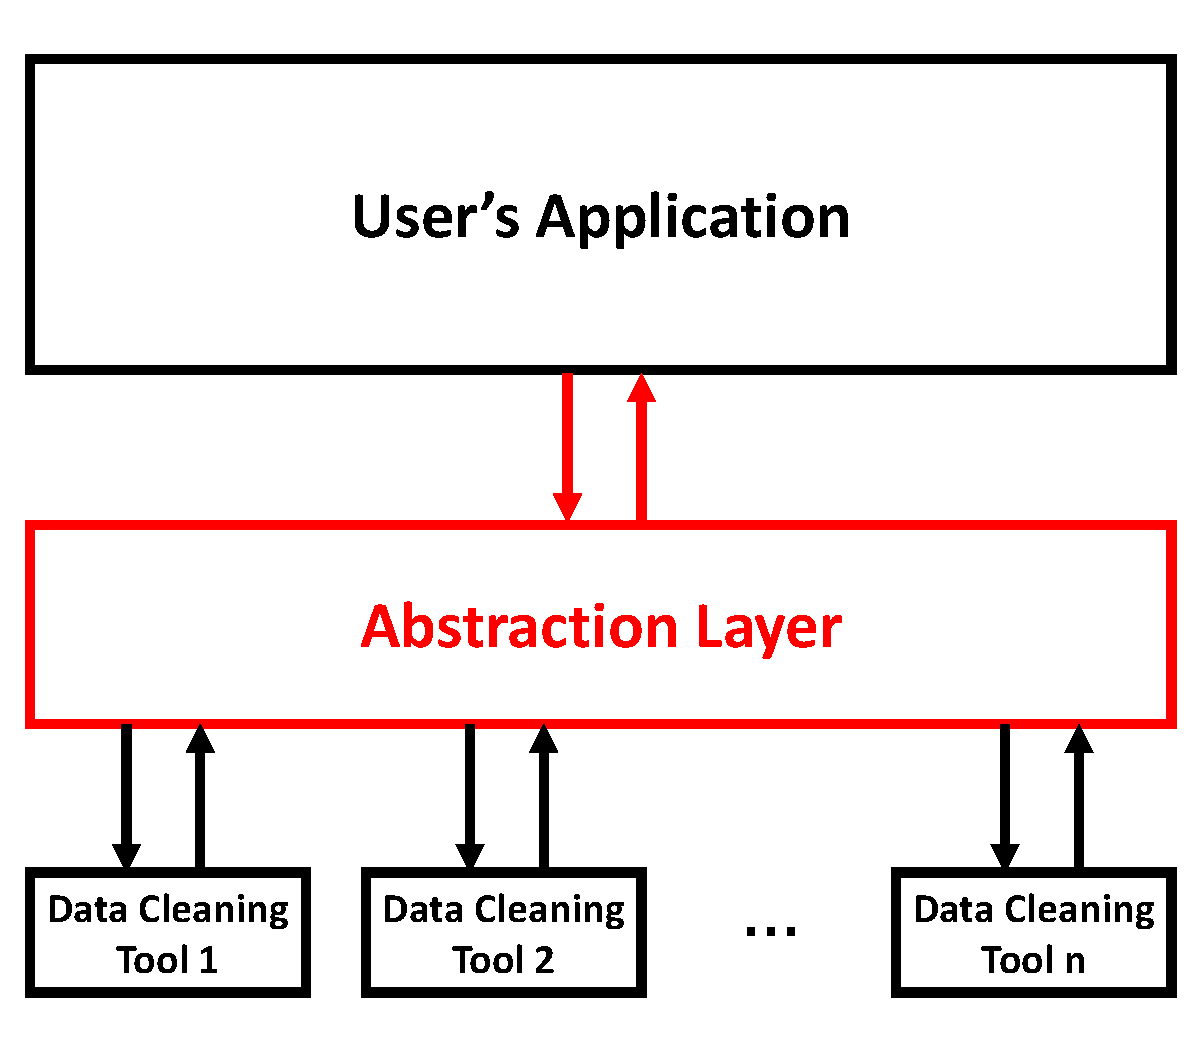
\includegraphics[scale=0.3]{attachments/architecture}
	\caption{The position of the abstraction layer in the architecture of the user's system.}
	\label{figure:architecture}
\end{figure}

\subsection{Overview}
The rest of this document is organized as follows. In Section~\ref{section:installation} we explain how the user can install the module. In Section 3 has introduced about input and output format and then some example are generated for better understanding.

\mohammad{complete this subsection}
%%%%%%%%%%%%%%%%%%%%%%%%%%%%%%%%%%%%%%%%%%%%%%%%%%%%


%%%%%%%%%%%%%%%%%%%%%%%%%%%%%%%%%%%%%%%%%%%%%%%%%%%%
\section{Installation}
\label{section:installation}

\subsection{Prerequisites}
To install the module, you need first to install followings:
\begin{itemize}
	\item Linux (Ubuntu/Debian recommended)
	\item Python 2.7
	\item Oracle Java 1.8
	\item Apache Ant 1.8.2+
	\item Postgres SQL 9.2+
\end{itemize}

\subsection{Setup}
the designed library has two main part, first part check the installation on the tools that supported by abstract layer and if it is needed the following tools will be install automatically and store in respect place that the layer is located.
For communicate and execute the installation the respect function is Considered:
\begin{lstlisting}
install_tools()
	
\end{lstlisting}
for working with second part of layer the function with the appropriate input should call that is introduced in the following section.
   
\mohammad{talk about how the user can use the installation function in the first place to installs and configures the tools. introduce the API function that installs and configures the tools.}
%%%%%%%%%%%%%%%%%%%%%%%%%%%%%%%%%%%%%%%%%%%%%%%%%%%%


%%%%%%%%%%%%%%%%%%%%%%%%%%%%%%%%%%%%%%%%%%%%%%%%%%%%
\section{Start to Work}

\subsection{Input}
For starting with abstract layer, required to make input configuration with the rules that is introduced by detail in the following.
Input configuration really is a dictionary that make by users and give to abstract layer as input and let functions to starts.This dictionary has two keys, the first one clarify type of the file and location of the file as path. In fact, for now the layer only support the files that generate with csv format but we will keep going to add other formats for future.
 
\mohammad{before introducing the template of your input configuration (look below), first start to talk generally about: (1) proper api function. (2) define the argument that it needs (input configuration, data cleaning job, or whatever you call it), then you have the following codes:}
\begin{lstlisting}[language=Python]
run_input = {
	"dataset": {
		"type": "csv",
		"param": ["the/address/of/your/file.csv"]
	},
	"tool": {
		"name": "tool name",
		"param": ["list of parameters wrt. to the tool name"]
	}
}
\end{lstlisting}

\mohammad{after the general template of the input object, start to explain each key and its proper values in a nested list:}
\begin{itemize}
	\item \textbf{dataset}. This part of the input configuration is responsible to describe the input dataset. it consists of two options:
	\begin{itemize}
		\item \textbf{type}. This option specifies the type of dataset. Currently the module only supports "csv" datasets.
		\item \textbf{param}. This option specifies the list of parameters that are needed for accessing the dataset. For csv datasets, this list contains only the path of dataset.
	\end{itemize}

	\item \textbf{tool}.
	the second part of the input configuration consist on the type of tool that user have plan to use it and parameters that each tool need for running.
	\begin{itemize}
		\item\textbf{name}.
		In this section the user clarify name of the tool which is want to use it.Currently "Nadeef" and "Dboost" covered by abstract layer.
	
		\item \textbf{param}
		This option specifies the parameters and entry of each tool regarding to the tool that has been chosen in the section before for tool's name.  
		
	\end{itemize}

\end{itemize}

Example for Nadeef:
\begin{lstlisting}

	run_input = {
				"dataset": {
				"type": "csv",
				"param": ["datasets/sample.csv"]
				},
				"tool": {
						"name": "nadeef",
						"param": [
						{
							"type": "fd",
							"value": ["title | brand_name"]
						}
								]
				}
			}
	
\end{lstlisting}
Example for Dboost:
\begin{lstlisting}

run_input = {
			"dataset": {
						"type": "csv",
						"param": ["datasets/sample.csv"]
					   },
					  "tool": {
						"name": "dboost",
						"param": ["--gaussian", "1", "--statistical", "1"]
							  }
					   }
\end{lstlisting}
\subsection{Output}
Regardless of data type and tools that is selected by user for data cleaning job, the abstract layer return constant output.
\begin{itemize}
	\item \textbf{Return:}
	user will receive one list as output that suspicious elements by row,column and old value return to user after execution.
	
	[row, column, suspicions value]
	 
\end{itemize}

\mohammad{just like the input subsection, write in this subsection.}
%%%%%%%%%%%%%%%%%%%%%%%%%%%%%%%%%%%%%%%%%%%%%%%%%%%%


%%%%%%%%%%%%%%%%%%%%%%%%%%%%%%%%%%%%%%%%%%%%%%%%%%%%
\bibliographystyle{unsrt}
\bibliography{attachments/bibliography}


\end{document}
%%%%%%%%%%%%%%%%%%%%%%%%%%%%%%%%%%%%%%%%%%%%%%%%%%%%